\section{Beamforming}\label{sec:theory:beam}

\begin{enumerate}
%  \item Explanation
%  \subitem straight line
%  \subitem phase shifting
%  \item Ideal calculation
%  \subitem Number of speakers
%  \subitem Distance of speakers
  \item Real-World behavior/limitations
  \subitem Real speaker distance
  \subitem Real speaker characteristics
\end{enumerate}

Beamforming is a concept used for emitting and receiving signals. It describes the technique of bundling a signal so it's only transmitted into or received from one direction. Because in this thesis beamforming is used with a speaker the following explanation will use an emitter as example but the calculations would work exactly the same for a receiver.\p
%
In order to produce the beamforming effect for one dimension you need multiple emitters arranged in one line.
If the receiver is far enough away from the emitters the directional vector of the waves can be viewed as parallel (See figure \dots). When the receiver is positioned directly in front of the emitters (\(0^\circ\)) all waves reach it at the same time (See figure \dots).
When the position of the receiver is rotated (\(\pm \varphi^\circ\)) the waves have to travel different distances. Therefore they reach the receiver with a phase shift (See figure \dots). Depending of the position of the receiver and distance of the emitters the waves will cancel each other out.\p
%
The difference in travel distance of two waves depending on the angle \(\varphi\) can be described as follows. \(d\) describes the spacing between the emitters.
%
\begin{align}
  l(\varphi) &= \sin \varphi \cdot d
\end{align}
%
Given the connection between distance $d$, time $t$ and velocity $v$. This equation can be used to calculate the phaseshift $\Phi$ between those two waves.
%
\begin{align}
  t(\varphi)     &= \frac{l}{v} = \frac{d}{v} \sin \varphi \\[1em]
  \Phi(\varphi)  &= \omega \cdot t = \frac{\omega}{v} d \cdot \sin \varphi \\[1em]
  \mathrm{with~} \lambda &= \frac{v}{f} \implies \frac{\omega}{v} = \frac{2\pi \cdot f}{v} = \frac{2\pi}{\lambda} \\[1em]
  \Phi(\varphi)  &= \frac{2\pi}{\lambda} d \cdot \sin \varphi \label{eq:theory:beam:single_phaseshift}
\end{align}
%
Equation \ref{eq:theory:beam:single_phaseshift} can also be used for a whole array of emitters, where $\Phi(\varphi)$ describes the phaseshift between two adjacent emitters. To get the phaseshift of the $n$th speaker relative to the first one ($n=0$) the phaseshifts $\Phi(\varphi)$ just need to be summed up.
%
\begin{align}
  \Phi(\varphi, n) &= n \cdot \frac{2\pi}{\lambda} d \cdot \sin \varphi
\end{align}
%
Given a set of two spherical emitter generating a cosine wave (\(s_e(t)\)), the received signal (\(s(t)\)) would look as shown in figure \ref{fig:theory:beam:time}.
%
\begin{figure}
  \centering
  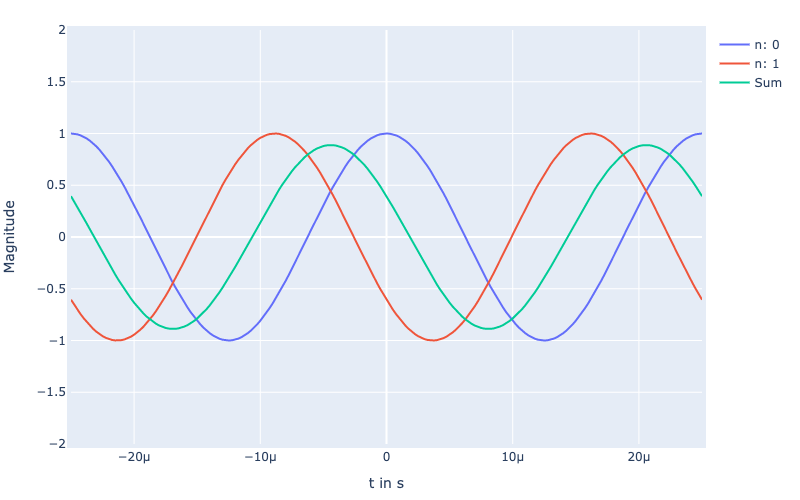
\includegraphics[height=\mediumheight]{src/assets/pictures/theory/beam_time_n2_45deg.png}
  \caption{Signals of every emitter in a phased array}
  \label{fig:theory:beam:time}
\end{figure}
%
\begin{align}
  s_e(t, \varphi, n) = \cos (\omega t + n \cdot \frac{2\pi}{\lambda} d \cdot \sin \varphi )\label{eq:theory:beam:sig}\\[1em]
  s(t, \varphi) = \sum_{n = 0}^{N} s_e(t, \varphi, n)
\end{align}
%
For a better analysis the resulting signal \(s(t, \varphi)\) is fourier transformed. Now the amplitude of the signal can be displayed depending on the position \(\varphi\) in a polar graph. The Amplitude is displayed in dB relative to the highest amplitude (See figure \ref{fig:theory:beam:n2_d.5}).\p
It can be observed, that the amplitude of the resulting signal is reduced the larger \(\varphi\) gets. Until both waves cancel each other out at \(90^\circ\).
%
\begin{figure}
  \centering
  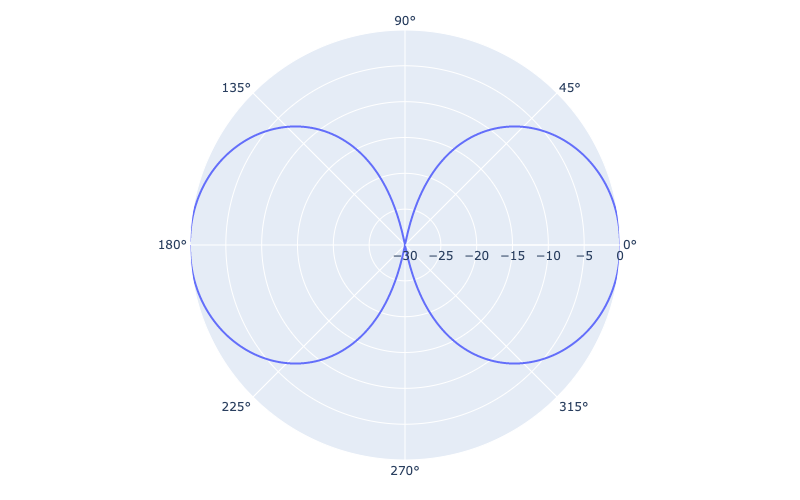
\includegraphics[height=\mediumheight]{src/assets/pictures/theory/beam_n2_d0.5.png}
  \caption{Phased array distribution characteristics ($d = \cfrac{1}{2}\lambda$, 2 emitters)}\label{fig:theory:beam:n2_d.5}
\end{figure}

\subsection{Distance between Emitters}

The beamforming characteristics can easily be influenced by the distance between the emitters, hence any changes in the phaseshift.
%As shown in equation \ref{eq:theory:beam:single_phaseshift} the phaseshift between two emitters depends on the distance between them. Therefore the beamforming characteristics can be easily influenced by this.
The ideal distance is half of the wavelength of the transmitted signal. With this spacing the two waves cancel each other out at exactly $90^\circ$ as shown in figure \ref{fig:theory:beam:n2_d.5}.\p
%
Figures \ref{fig:theory:beam:d} and \ref{fig:theory:beam:n2_d.5} show the beamforming characteristics of a phased array with $2$ emitters and a distance of $\cfrac{1}{4}\lambda$, $\cfrac{1}{2}\lambda$, $\lambda$, and $2\lambda$. The graph shows that using a smaller distance than $\frac{1}{2} \lambda$ makes the beamforming effect slowly disappear while a higher distance introduces a side beam at $\pm 90^\circ$. If the distance is further increased, the side beams split up and a new one emerges at $\pm 90^\circ$.
%
\begin{figure}[ht]
  \begin{subfigure}[b]{0.32\textwidth}
    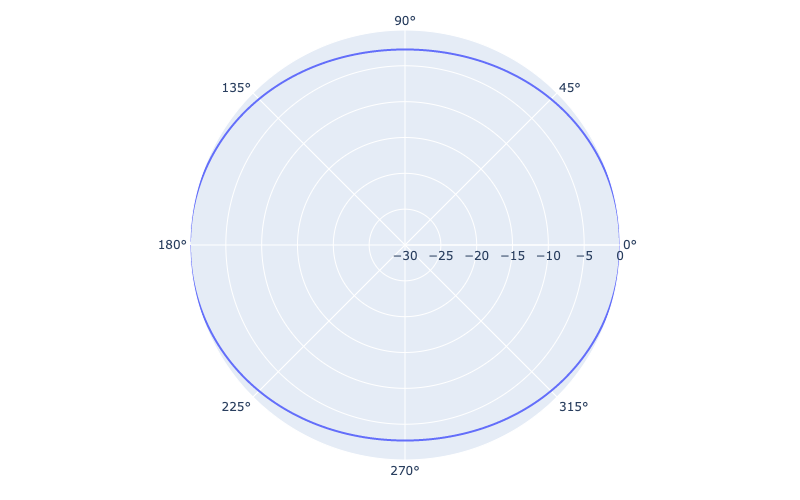
\includegraphics[width=\textwidth]{src/assets/pictures/theory/beam_n2_d0.25.png}
    \caption{$d = \cfrac{1}{4}\lambda$}
    \label{fig:theory:beam:d.25}
  \end{subfigure}
  \hfill
  \begin{subfigure}[b]{0.32\textwidth}
    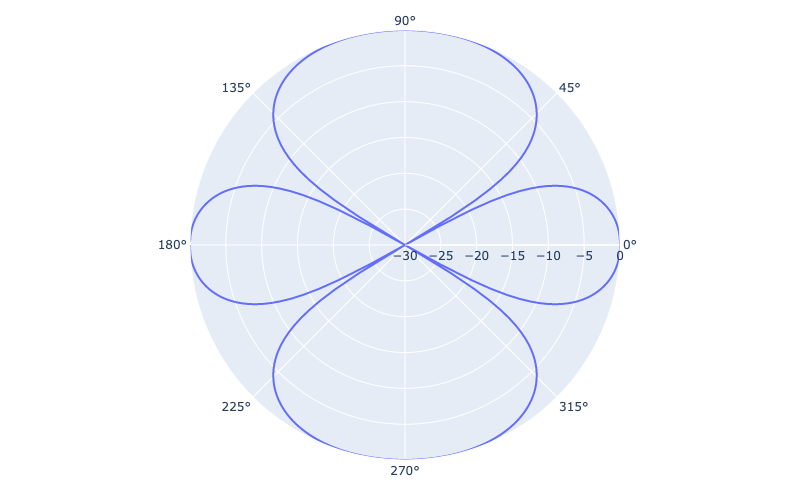
\includegraphics[width=\textwidth]{src/assets/pictures/theory/beam_n2_d1.png}
    \caption{$d = \lambda$}
    \label{fig:theory:beam:d1}
  \end{subfigure}
  \hfill
  \begin{subfigure}[b]{0.32\textwidth}
    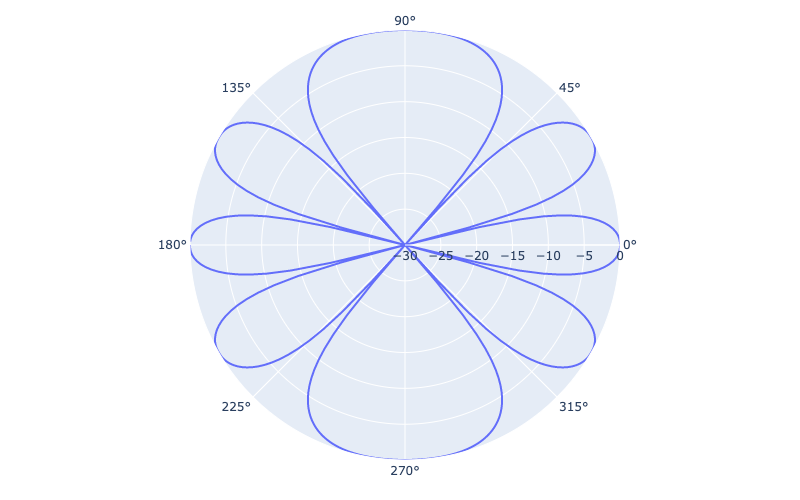
\includegraphics[width=\textwidth]{src/assets/pictures/theory/beam_n2_d2.png}
    \caption{$d = 2\lambda$}
    \label{fig:theory:beam:d2}
  \end{subfigure}
  \caption{Beamforming characteristics depending on the distance between emitters}
  \label{fig:theory:beam:d}
\end{figure}
%
\subsection{Number of Emitters}

Figure \dots shows the beamforming characteristics of a phased array with $2$, $5$ and $20$ emitters. The distance between the emitters is set to $\frac{1}{2} \lambda$. From the graphs can be observed, that by increasing the number of emitters the generated beam gets narrower. However a higher number of emitters also introduces new side beams with a smaller amplitude. The amplitude of the side beams decreases the larger the number of emitters.
%
\begin{figure}[ht]
  \begin{subfigure}[b]{0.32\textwidth}
    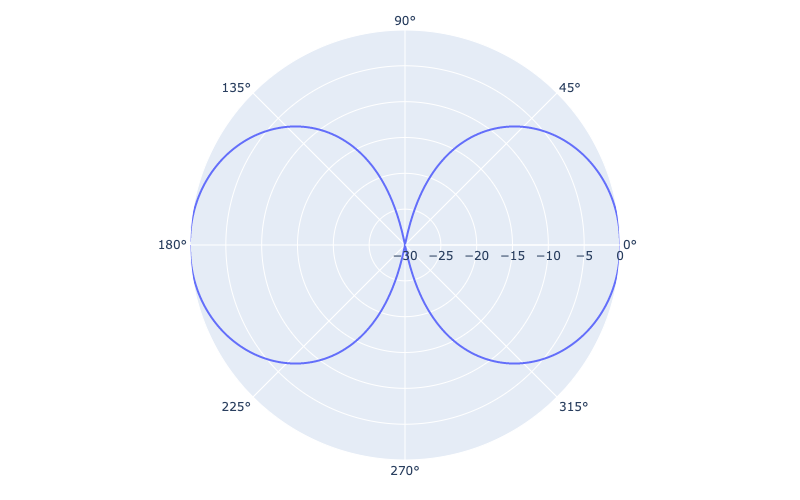
\includegraphics[width=\textwidth]{src/assets/pictures/theory/beam_n2_d0.5.png}
    \caption{2 emitters}
    \label{fig:theory:beam:num_2}
  \end{subfigure}
  \hfill
  \begin{subfigure}[b]{0.32\textwidth}
    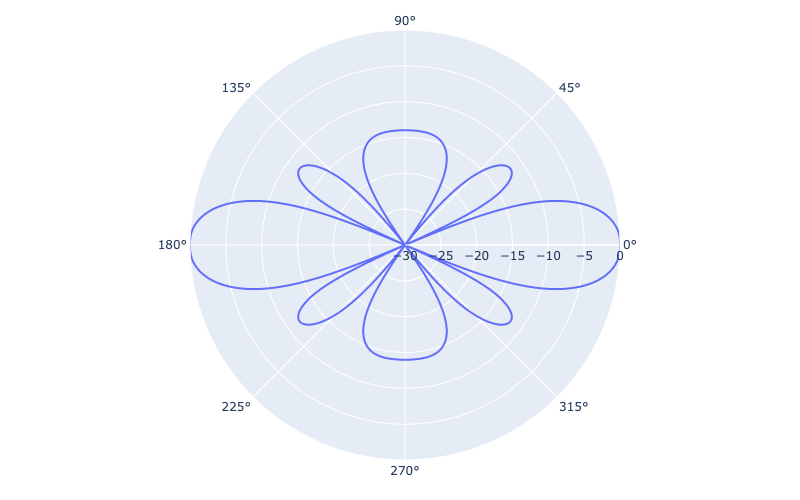
\includegraphics[width=\textwidth]{src/assets/pictures/theory/beam_n5.png}
    \caption{5 emitters}
    \label{fig:theory:beam:num_5}
  \end{subfigure}
  \hfill
  \begin{subfigure}[b]{0.32\textwidth}
    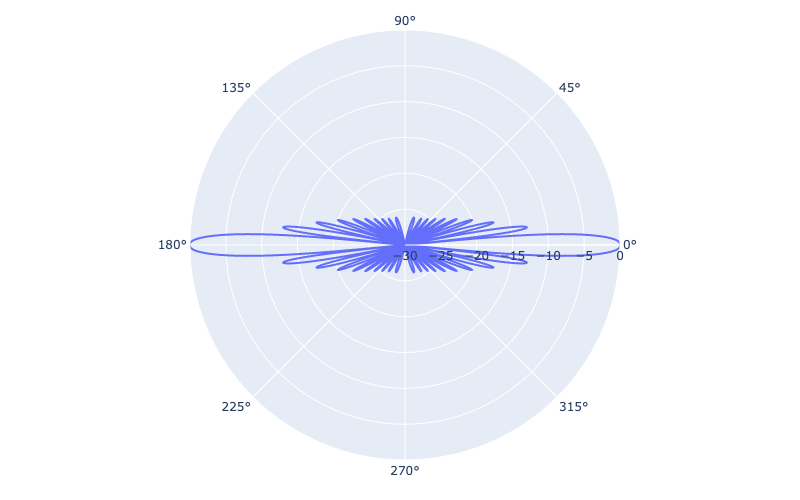
\includegraphics[width=\textwidth]{src/assets/pictures/theory/beam_n20.png}
    \caption{20 emitters}
    \label{fig:theory:beam:num_20}
  \end{subfigure}
  \caption{Beamforming characteristics depending on the number of emitters}
  \label{fig:theory:beam:num}
\end{figure}
%
\subsection{Dispersion Characteristics of Emitters}
For the calculations above the emitters are assumed to be isotropic radiators. In the real world a speaker has some form of direction characteristic. The exact behavior is highly dependent of the signal frequency. A higher frequency usually means more directivity.\p
%
Figure \dots shows the dispersion characteristics of the ultrasonic transducer used in this project. This behavior can be modelled into equation \ref{eq:theory:beam:sig} as follows:
%
\begin{align}
  s_e(t, \varphi, n) &= \dots
\end{align}
%
The resulting characteristics of the phased array compared to the result with isotropic radiators are shown in figure \dots. It can be observed, that \dots